\documentclass{article}
\usepackage{color}
\usepackage[margin=1in]{geometry}
\usepackage[utf8]{inputenc}
\usepackage{amsmath}
\usepackage{amsfonts}
\usepackage{amssymb}
\usepackage{graphicx} % Not used here, but often useful

% Define matrix and vector commands for convenience
\newcommand{\mat}[1]{\begin{bmatrix} #1 \end{bmatrix}}
\newcommand{\vect}[1]{\begin{bmatrix} #1 \end{bmatrix}}
\title{PS8}
\author{Giacomo Cappelletto}
\begin{document}

\maketitle

\section*{1}
\subsection*{A}


\[
	A - \lambda I = \mat{ 2 - \lambda & -1 & -2 \\ 0 & 1 - \lambda & -2 \\ 0 & -2 & 1 - \lambda }
\]
\[
	\begin{aligned}
		\det(A - \lambda I) & = (2 - \lambda) \det \begin{pmatrix} 1 - \lambda & -2 \\ -2 & 1 - \lambda \end{pmatrix} - 0 + 0 \\
		                    & = (2 - \lambda) \left[ (1 - \lambda)(1 - \lambda) - (-2)(-2) \right]                            \\
		                    & = (2 - \lambda) \left[ (1 - \lambda)^2 - 4 \right]                                              \\
		                    & = (2 - \lambda) \left[ 1 - 2\lambda + \lambda^2 - 4 \right]                                     \\
		                    & = (2 - \lambda) (\lambda^2 - 2\lambda - 3)
	\end{aligned}
\]
\[
	(2 - \lambda)(\lambda - 3)(\lambda + 1) = 0
\]
The eigenvalues are $\mathbf{\lambda_1 = 2}$, $\mathbf{\lambda_2 = 3}$, and $\mathbf{\lambda_3 = -1}$.


\textbf{For $\lambda_1 = 2$:}
\[
	\mat{ 0 & -1 & -2 \\ 0 & -1 & -2 \\ 0 & -2 & -1 } \vect{x \\ y \\ z} = \vect{0 \\ 0 \\ 0}
\]
\[
	\mat{ 0 & -1 & -2 \\ 0 & -1 & -2 \\ 0 & -2 & -1 }
	\xrightarrow{\substack{R_2 = R_2 - R_1 \\ R_3 = R_3 - 2R_1}}
	\mat{ 0 & -1 & -2 \\ 0 & 0 & 0 \\ 0 & 0 & 3 }
	\xrightarrow{R_1 \leftrightarrow R_3, R_3 \to R_2} % Reorder rows
	\mat{ 0 & 0 & 3 \\ 0 & -1 & -2 \\ 0 & 0 & 0 }
	\xrightarrow{\substack{R_1 = \frac{1}{3}R_1 \\ R_2 = -R_2}}
	\mat{ 0 & 0 & 1 \\ 0 & 1 & 2 \\ 0 & 0 & 0 }
	\xrightarrow{R_2 = R_2 - 2R_1} % Get RREF
	\mat{ 0 & 1 & 0 \\ 0 & 0 & 1 \\ 0 & 0 & 0 }
\]
\[
	\therefore \text{A basis eigenvector for} \lambda_2 = 3 \text{is}
	\begin{bmatrix}
		1 \\ 0 \\ 0
	\end{bmatrix}
\]


\textbf{For $\lambda_2 = 3$:}
\[
	\mat{ -1 & -1 & -2 \\ 0 & -2 & -2 \\ 0 & -2 & -2 } \vect{x \\ y \\ z} = \vect{0 \\ 0 \\ 0}
\]
\[
	\mat{ -1 & -1 & -2 \\ 0 & -2 & -2 \\ 0 & -2 & -2 }
	\xrightarrow{R_3 = R_3 - R_2}
	\mat{ -1 & -1 & -2 \\ 0 & -2 & -2 \\ 0 & 0 & 0 }
	\xrightarrow{R_2 = -\frac{1}{2}R_2}
	\mat{ -1 & -1 & -2 \\ 0 & 1 & 1 \\ 0 & 0 & 0 }
	\xrightarrow{R_1 = R_1 + R_2}
	\mat{ -1 & 0 & -1 \\ 0 & 1 & 1 \\ 0 & 0 & 0 }
	\xrightarrow{R_1 = -R_1}
	\mat{ 1 & 0 & 1 \\ 0 & 1 & 1 \\ 0 & 0 & 0 }
\]
\[
	\therefore \text{A basis eigenvector for} \lambda_2 = 3 \text{is}
	\begin{bmatrix}
		-1 \\ -1 \\ 1
	\end{bmatrix}
\]

\textbf{For $\lambda_3 = -1$:}
\[
	\mat{ 3 & -1 & -2 \\ 0 & 2 & -2 \\ 0 & -2 & 2 } \vect{x \\ y \\ z} = \vect{0 \\ 0 \\ 0}
\]
\[
	\mat{ 3 & -1 & -2 \\ 0 & 2 & -2 \\ 0 & -2 & 2 }
	\xrightarrow{R_3 = R_3 + R_2}
	\mat{ 3 & -1 & -2 \\ 0 & 2 & -2 \\ 0 & 0 & 0 }
	\xrightarrow{R_2 = \frac{1}{2}R_2}
	\mat{ 3 & -1 & -2 \\ 0 & 1 & -1 \\ 0 & 0 & 0 }
	\xrightarrow{R_1 = R_1 + R_2}
	\mat{ 3 & 0 & -3 \\ 0 & 1 & -1 \\ 0 & 0 & 0 }
	\xrightarrow{R_1 = \frac{1}{3}R_1}
	\mat{ 1 & 0 & -1 \\ 0 & 1 & -1 \\ 0 & 0 & 0 }
\]
\[
	\therefore \text{A basis eigenvector for} \lambda_3 = -1 \text{is}
	\begin{bmatrix}
		1 \\ 1 \\ 1
	\end{bmatrix}
\]

\subsection*{B}

\[
	A = \mat{ 2 & -1 & -2 \\ 0 & 1 & -2 \\ 0 & -2 & 1 }
\]
\[
	\begin{aligned}
		\det(A) & = 2 \cdot \det \begin{pmatrix} 1 & -2 \\ -2 & 1 \end{pmatrix} - 0 \cdot \det \begin{pmatrix} -1 & -2 \\ -2 & 1 \end{pmatrix} + 0 \cdot \det \begin{pmatrix} -1 & -2 \\ 1 & -2 \end{pmatrix} \\
		        & = 2 \left[ (1)(1) - (-2)(-2) \right] - 0 + 0                                                                                                                                                \\
		        & = 2 [1 - 4]                                                                                                                                                                                 \\
		        & = 2 [-3]                                                                                                                                                                                    \\
		        & = \mathbf{-6}
	\end{aligned}
\]
\[
	\det(A) = -6
\]


\subsection*{C}


\[
	\lambda_1 \times \lambda_2 \times \lambda_3 = (2) \times (3) \times (-1) = \mathbf{-6}
\]

\subsection*{D}

Matlab standardizes the eigenvectors by normalizing them to have a  length (norm) of 1, ensuring a unique representative for each eigenvector direction. The calculated eigenvectors are simply multiples of the ones given by Matlab

\section*{2}
\subsection*{A}

\[
	B - \lambda I = \mat{ 1 - \lambda & -1 & 1 \\ 2 & -2 - \lambda & 1 \\ 2 & -1 & -\lambda }
\]
\[
	\begin{aligned}
		\det(B - \lambda I) & = (1 - \lambda) \det \begin{pmatrix} -2 - \lambda & 1 \\ -1 & -\lambda \end{pmatrix} - (-1) \det \begin{pmatrix} 2 & 1 \\ 2 & -\lambda \end{pmatrix} + 1 \det \begin{pmatrix} 2 & -2 - \lambda \\ 2 & -1 \end{pmatrix} \\
		                    & = (1 - \lambda) [ (-\lambda)(-2 - \lambda) - (1)(-1) ] + 1 [ (2)(-\lambda) - (1)(2) ] + 1 [ (2)(-1) - (-2 - \lambda)(2) ]                                                                                              \\
		                    & = (1 - \lambda) [ 2\lambda + \lambda^2 + 1 ] + [ -2\lambda - 2 ] + [ -2 - (-4 - 2\lambda) ]                                                                                                                            \\
		                    & = (1 - \lambda) (\lambda + 1)^2 - 2\lambda - 2 + [ -2 + 4 + 2\lambda ]                                                                                                                                                 \\
		                    & = (1 - \lambda) (\lambda + 1)^2 - 2\lambda - 2 + 2 + 2\lambda                                                                                                                                                          \\
		                    & = (1 - \lambda) (\lambda + 1)^2                                                                                                                                                                                        \\
		                    & = -(\lambda - 1)(\lambda + 1)^2
	\end{aligned}
\]
Setting $\det(B - \lambda I) = 0$, the eigenvalues are $\mathbf{\lambda_1 = 1}$ (\(k=1\)) and $\mathbf{\lambda_2 = -1}$ (\(k=2\)).

\textbf{For $\lambda_1 = 1$:}
\[
	\mat{ 0 & -1 & 1 \\ 2 & -3 & 1 \\ 2 & -1 & -1 } \vect{x \\ y \\ z} = \vect{0 \\ 0 \\ 0}
\]
\[
	\mat{ 0 & -1 & 1 \\ 2 & -3 & 1 \\ 2 & -1 & -1 }
	\xrightarrow{R_1 \leftrightarrow R_2}
	\mat{ 2 & -3 & 1 \\ 0 & -1 & 1 \\ 2 & -1 & -1 }
	\xrightarrow{R_3 = R_3 - R_1}
	\mat{ 2 & -3 & 1 \\ 0 & -1 & 1 \\ 0 & 2 & -2 }
	\xrightarrow{R_3 = R_3 + 2R_2}
	\mat{ 2 & -3 & 1 \\ 0 & -1 & 1 \\ 0 & 0 & 0 }
\]
\[
	\xrightarrow{R_2 = -R_2}
	\mat{ 2 & -3 & 1 \\ 0 & 1 & -1 \\ 0 & 0 & 0 }
	\xrightarrow{R_1 = R_1 + 3R_2}
	\mat{ 2 & 0 & -2 \\ 0 & 1 & -1 \\ 0 & 0 & 0 }
	\xrightarrow{R_1 = \frac{1}{2}R_1}
	\mat{ 1 & 0 & -1 \\ 0 & 1 & -1 \\ 0 & 0 & 0 }
\]
The eigenvectors are $t \vect{1 \\ 1 \\ 1}$.
\[
	\therefore \text{A basis eigenvector for } \lambda_1 = 1 \text{ is } \vect{1 \\ 1 \\ 1}
\]

\textbf{For $\lambda_2 = -1$:}
\[
	\mat{ 2 & -1 & 1 \\ 2 & -1 & 1 \\ 2 & -1 & 1 } \vect{x \\ y \\ z} = \vect{0 \\ 0 \\ 0}
\]
\[
	\mat{ 2 & -1 & 1 \\ 2 & -1 & 1 \\ 2 & -1 & 1 }
	\xrightarrow{\substack{R_2 = R_2 - R_1 \\ R_3 = R_3 - R_1}}
	\mat{ 2 & -1 & 1 \\ 0 & 0 & 0 \\ 0 & 0 & 0 }
\]
The eigenvectors are $\vect{ \frac{1}{2}s - \frac{1}{2}t \\ s \\ t } = s \vect{1/2 \\ 1 \\ 0} + t \vect{-1/2 \\ 0 \\ 1}$.
We can choose integer basis vectors by setting $(s=2, t=0)$ and $(s=0, t=2)$.
\[
	\therefore \text{Basis eigenvectors for } \lambda_2 = -1 \text{ are } \vect{1 \\ 2 \\ 0} \text{ and } \vect{-1 \\ 0 \\ 2}
\]

\subsection*{B}

Yes, the first column of $V$, matches our hand-calculated eigenvector $\mathbf{v_1 = \vect{1 \\ 1 \\ 1}}$ associated with the eigenvalue $\lambda_1 = 1$.\\
The second and third columns of $V$ do not directly match our hand-calculated basis vectors $\mathbf{v_2 = \vect{1 \\ 2 \\ 0}}$ or $\mathbf{v_3 = \vect{-1 \\ 0 \\ 2}}$. Both sets of vectors form a basis for the eigenspace associated with the eigenvalue $\lambda_2 = -1$. Matlab provides a different basis than the one we found by hand.

\section*{3}

\[
	\begin{aligned}
		\det(C - \lambda I) & = -2 \det \begin{pmatrix} 7 & 1 \\ 11 & 7 - \lambda \end{pmatrix} + (-\lambda) \det \begin{pmatrix} -2 - \lambda & 1 \\ -8 & 7 - \lambda \end{pmatrix} - (-2) \det \begin{pmatrix} -2 - \lambda & 7 \\ -8 & 11 \end{pmatrix} \\
		                    & = -2 [ 7(7 - \lambda) - (1)(11) ] - \lambda [ (-2 - \lambda)(7 - \lambda) - (1)(-8) ] + 2 [ (-2 - \lambda)(11) - (7)(-8) ]                                                                                                   \\
		                    & = -2 [ 49 - 7\lambda - 11 ] - \lambda [ -14 + 2\lambda - 7\lambda + \lambda^2 + 8 ] + 2 [ -22 - 11\lambda + 56 ]                                                                                                             \\
		                    & = -2 [ 38 - 7\lambda ] - \lambda [ \lambda^2 - 5\lambda - 6 ] + 2 [ 34 - 11\lambda ]                                                                                                                                         \\
		                    & = -76 + 14\lambda - \lambda^3 + 5\lambda^2 + 6\lambda + 68 - 22\lambda                                                                                                                                                       \\
		                    & = -\lambda^3 + 5\lambda^2 + (14 + 6 - 22)\lambda + (-76 + 68)                                                                                                                                                                \\
		                    & = -\lambda^3 + 5\lambda^2 - 2\lambda - 8
	\end{aligned}
\]
The characteristic equation is $-\lambda^3 + 5\lambda^2 - 2\lambda - 8 = 0$, or $\lambda^3 - 5\lambda^2 + 2\lambda + 8 = 0$.
Let $P(\lambda) = \lambda^3 - 5\lambda^2 + 2\lambda + 8$.
Possible rational roots: $\pm 1, \pm 2, \pm 4, \pm 8$.
$P(-1) = -1 - 5 - 2 + 8 = 0$.
$P(2) = 8 - 5(4) + 2(2) + 8 = 8 - 20 + 4 + 8 = 0$.
$P(4) = 64 - 5(16) + 2(4) + 8 = 64 - 80 + 8 + 8 = 0$.
The eigenvalues are $\mathbf{\lambda_1 = -1}$, $\mathbf{\lambda_2 = 2}$, $\mathbf{\lambda_3 = 4}$.

\textbf{For $\lambda_1 = -1$:}
\[
	\mat{ -1 & 7 & 1 \\ 2 & 1 & -2 \\ -8 & 11 & 8 } \vect{x \\ y \\ z} = \vect{0 \\ 0 \\ 0}
\]
\[
	\mat{ -1 & 7 & 1 \\ 2 & 1 & -2 \\ -8 & 11 & 8 }
	\xrightarrow{\substack{R_2 = R_2 + 2R_1 \\ R_3 = R_3 - 8R_1}}
	\mat{ -1 & 7 & 1 \\ 0 & 15 & 0 \\ 0 & -45 & 0 }
	\xrightarrow{R_2 = \frac{1}{15}R_2}
	\mat{ -1 & 7 & 1 \\ 0 & 1 & 0 \\ 0 & -45 & 0 }
\]
\[
	\xrightarrow{\substack{R_1 = R_1 - 7R_2 \\ R_3 = R_3 + 45R_2}}
	\mat{ -1 & 0 & 1 \\ 0 & 1 & 0 \\ 0 & 0 & 0 }
	\xrightarrow{R_1 = -R_1}
	\mat{ 1 & 0 & -1 \\ 0 & 1 & 0 \\ 0 & 0 & 0 }
\]
\[
	\therefore \text{A basis eigenvector for } \lambda_1 = -1 \text{ is } \vect{1 \\ 0 \\ 1}
\]

\textbf{For $\lambda_2 = 2$:}

\[
	\mat{ -4 & 7 & 1 \\ 2 & -2 & -2 \\ -8 & 11 & 5 } \vect{x \\ y \\ z} = \vect{0 \\ 0 \\ 0}
\]

\[
	\mat{ -4 & 7 & 1 \\ 2 & -2 & -2 \\ -8 & 11 & 5 }
	\xrightarrow{R_1 \leftrightarrow R_2}
	\mat{ 2 & -2 & -2 \\ -4 & 7 & 1 \\ -8 & 11 & 5 }
	\xrightarrow{R_1 = \frac{1}{2}R_1}
	\mat{ 1 & -1 & -1 \\ -4 & 7 & 1 \\ -8 & 11 & 5 }
\]
\[
	\xrightarrow{\substack{R_2 = R_2 + 4R_1 \\ R_3 = R_3 + 8R_1}}
	\mat{ 1 & -1 & -1 \\ 0 & 3 & -3 \\ 0 & 3 & -3 }
	\xrightarrow{R_2 = \frac{1}{3}R_2}
	\mat{ 1 & -1 & -1 \\ 0 & 1 & -1 \\ 0 & 3 & -3 }
\]
\[
	\xrightarrow{\substack{R_1 = R_1 + R_2 \\ R_3 = R_3 - 3R_2}}
	\mat{ 1 & 0 & -2 \\ 0 & 1 & -1 \\ 0 & 0 & 0 }
\]
\[
	\therefore \text{A basis eigenvector for } \lambda_2 = 2 \text{ is } \vect{2 \\ 1 \\ 1}
\]

\textbf{For $\lambda_3 = 4$:}
\[
	\mat{ -6 & 7 & 1 \\ 2 & -4 & -2 \\ -8 & 11 & 3 } \vect{x \\ y \\ z} = \vect{0 \\ 0 \\ 0}
\]
\[
	\mat{ -6 & 7 & 1 \\ 2 & -4 & -2 \\ -8 & 11 & 3 }
	\xrightarrow{R_1 \leftrightarrow R_2}
	\mat{ 2 & -4 & -2 \\ -6 & 7 & 1 \\ -8 & 11 & 3 }
	\xrightarrow{R_1 = \frac{1}{2}R_1}
	\mat{ 1 & -2 & -1 \\ -6 & 7 & 1 \\ -8 & 11 & 3 }
\]
\[
	\xrightarrow{\substack{R_2 = R_2 + 6R_1 \\ R_3 = R_3 + 8R_1}}
	\mat{ 1 & -2 & -1 \\ 0 & -5 & -5 \\ 0 & -5 & -5 }
	\xrightarrow{R_2 = -\frac{1}{5}R_2}
	\mat{ 1 & -2 & -1 \\ 0 & 1 & 1 \\ 0 & -5 & -5 }
\]
\[
	\xrightarrow{\substack{R_1 = R_1 + 2R_2 \\ R_3 = R_3 + 5R_2}}
	\mat{ 1 & 0 & 1 \\ 0 & 1 & 1 \\ 0 & 0 & 0 }
\]
\[
	\therefore \text{A basis eigenvector for } \lambda_3 = 4 \text{ is } \vect{-1 \\ -1 \\ 1}
\]


\section*{4}
\subsection*{A}

\[
	D - \lambda I = \mat{ 2 - \lambda & 0 & 0 \\ 0 & 2 - \lambda & 1 \\ 0 & 0 & 2 - \lambda }
\]
\[
	\det(D - \lambda I) = (2 - \lambda)(2 - \lambda)(2 - \lambda) = (2 - \lambda)^3
\]
Setting $\det(D - \lambda I) = 0$, we get $(2 - \lambda)^3 = 0$.
The only eigenvalue is $\mathbf{\lambda = 2}$ with \(k=3\)

\textbf{For $\lambda = 2$:}
\[
	\mat{ 0 & 0 & 0 \\ 0 & 0 & 1 \\ 0 & 0 & 0 } \vect{x \\ y \\ z} = \vect{0 \\ 0 \\ 0}
\]
The eigenvectors are of the form $ t_1 \vect{1 \\ 0 \\ 0} + t_2 \vect{0 \\ 1 \\ 0}$.
The eigenspace is 2-dimensional ($k=2$).
\[
	\therefore \text{Basis eigenvectors for } \lambda = 2 \text{ are } \vect{1 \\ 0 \\ 0} \text{ and } \vect{0 \\ 1 \\ 0}
\]

\subsection*{B}

No, the number of eigenvectors reported by Matlab (3 columns in V) does not match the number of linearly independent eigenvectors found in the hand-derived calculations (2 basis vectors). The hand calculation found that the eigenspace for $\lambda=2$ is only 2-dimensional, meaning a basis consists of exactly two linearly independent eigenvectors.

\section*{5}

\subsection*{B}


\begin{verbatim}
	clear all;
	close all;
	
	
	% -- Default matrix A  (you can change this matrix A !!)
	
	
	A  =  [  2,-1,-1;
			 -1,2,-1;
			 -1,-1,2]
	
	
	% -- Select the eigenvector to plot
	
	eigvec_to_plot = 1;   % -- This is associated with:  lambda1 = 0
	%eigvec_to_plot = 2;   % -- This is associated with:  lambda2 = 3
	%eigvec_to_plot = 3;   % -- This is associated with:  lambda3 = 3
	
	
	disp('The eigenvalues and eigenvectors of matrix A are:')
	[V,D] = eig(A)
	
	% -- Define cube
	
	shift_x = 0;
	shift_y = 0;
	shift_z = 0;
	
	x1 = [0 1 1 0 0 1 1 0] + shift_x;
	x2 = [0 0 0 0 1 1 1 1] + shift_y;
	x3 = [0 0 1 1 0 0 1 1] + shift_z;
	
	% -- Define x
	x = [x1;  x2;  x3];
	
	% -- Calculate transformation
	y = A*x;
	
	% -- Housekeeping duties
	xmin = -2;
	xmax = 2;
	ymin = -2;
	ymax = 2;
	zmin = -2;
	zmax = 2;
	
	% -- Plot data points (preimage and image)
	
	figure
	
	for count = 1:1:length(x1)
		preimage_handle(count) = plot3(x(1,count), x(2,count), x(3,count), '.');
	
	
	
		if count == 1
			set(preimage_handle(count), 'Color', 'red', 'MarkerSize', 50, 'Linewidth', 5);
		else
	
			set(preimage_handle(count), 'Color', 'black', 'MarkerSize', 15, 'Linewidth', 5);
		end
	end
	
	
	% --  Plot one face of the preimage and its corresponding image
	
	preimageFace_handle(1) = patch(x(1, 1:4), x(2, 1:4), x(3, 1:4),  4);
	preimageFace_handle(2) = patch(x(1, 5:8), x(2, 5:8), x(3, 5:8),  4);
	preimageFace_handle(3) = patch(x(1, [1 4 8 5] ), x(2, [1 4 8 5]), x(3, [1 4 8 5]),  4);
	preimageFace_handle(4) = patch(x(1, [1 2 6 5]), x(2, [1 2 6 5]), x(3, [1 2 6 5]),  4);
	
	set(preimageFace_handle(1), 'FaceColor', 'blue', 'FaceAlpha', 1);
	set(preimageFace_handle(2), 'FaceColor', 'green', 'FaceAlpha', 0.2);
	set(preimageFace_handle(3), 'FaceColor', 'yellow', 'FaceAlpha', 0.2);
	set(preimageFace_handle(4), 'FaceColor', 'red', 'FaceAlpha', 0.2);
	
	
	% -- Emphasize the x, y, z-axexs
	%line([0 xmax], [0 0], [0 0], 'Color', 'black', 'Linestyle', '-.', 'Linewidth', 2);  % -- x-axis
	%line([0 0], [0 ymax], [0 0], 'Color', 'black', 'Linestyle', '-', 'Linewidth', 2);  % -- y-axis
	%line([0 0], [0 0], [0 zmax], 'Color', 'black', 'Linestyle', 'x', 'Linewidth', 2);  % -- z-axis
	
	eig_scale = 3;
	% -- Plot eigenvector #2
	line('XData', eig_scale.*[0 V(1,eigvec_to_plot)], 'YData', eig_scale.*[0 V(2,eigvec_to_plot)], 'ZData', eig_scale.*[0 V(3,eigvec_to_plot)], 'Color', 'black', 'Linestyle', '-.', 'Linewidth', 2);
	
	axis square;
	grid on;
	xlabel('x-axis', 'FontName', 'Arial', 'FontSize', 15);
	ylabel('y-axis', 'FontName', 'Arial', 'FontSize', 15);
	zlabel('z-axis', 'FontName', 'Arial', 'FontSize', 15);
	axis([xmin  xmax  ymin  ymax  zmin  zmax]   );
	hold off
	title('The pre-image before transformation by A')
	
	
	
	% \\\\\\\\\\\\\\\\\\\\\\\\\\\\\\\\\\\\\\\\\\\\\\\\\\\\
	%   Figure 2:  Plot the transformed image
	% \\\\\\\\\\\\\\\\\\\\\\\\\\\\\\\\\\\\\\\\\\\\\\\\
	
	xmin2 = -5;
	xmax2 = 5;
	ymin2 = -5;
	ymax2 = 5;
	zmin2 = -5;
	zmax2 = 5;
	
	
	figure
	
	for count = 1:1:length(x1)
		%preimage_handle(count) = plot3(x(1,count), x(2,count), x(3,count), '.');
		%hold on;
		image_handle(count) = plot3(y(1,count), y(2,count), y(3,count), 'o');
		hold on;
	
		if count == 1
				%set(preimage_handle(count), 'Color', 'red', 'MarkerSize', 50, 'Linewidth', 5);
				set(image_handle(count), 'Color', 'red', 'MarkerSize', 30, 'Linewidth', 1);
		else
	
			%set(preimage_handle(count), 'Color', 'black', 'MarkerSize', 15, 'Linewidth', 5);
			set(image_handle(count), 'Color', 'black', 'MarkerSize', 10, 'Linewidth', 5);
		end
	end
	
	
	% --  Plot one face of the preimage and its corresponding image
	
	% preimageFace_handle(1) = patch(x(1, 1:4), x(2, 1:4), x(3, 1:4),  4);
	% preimageFace_handle(2) = patch(x(1, 5:8), x(2, 5:8), x(3, 5:8),  4);
	% preimageFace_handle(3) = patch(x(1, [1 4 8 5] ), x(2, [1 4 8 5]), x(3, [1 4 8 5]),  4);
	% preimageFace_handle(4) = patch(x(1, [1 2 6 5]), x(2, [1 2 6 5]), x(3, [1 2 6 5]),  4);
	%
	% set(preimageFace_handle(1), 'FaceColor', 'blue', 'FaceAlpha', 1);
	% set(preimageFace_handle(2), 'FaceColor', 'green', 'FaceAlpha', 0.2);
	% set(preimageFace_handle(3), 'FaceColor', 'yellow', 'FaceAlpha', 0.2);
	% set(preimageFace_handle(4), 'FaceColor', 'red', 'FaceAlpha', 0.2);
	
	imageFace_handle(1) = patch(y(1, 1:4), y(2, 1:4), y(3, 1:4),  4);
	imageFace_handle(2) = patch(y(1, 5:8), y(2, 5:8), y(3, 5:8),  4);
	imageFace_handle(3) = patch(y(1, [1 4 8 5]), y(2, [1 4 8 5]), y(3, [1 4 8 5]),  4);
	imageFace_handle(4) = patch(y(1, [1 2 6 5]), y(2, [1 2 6 5]), y(3, [1 2 6 5]),  4);
	
	set(imageFace_handle(1), 'FaceColor', 'blue', 'FaceAlpha', 0.2);
	set(imageFace_handle(2), 'FaceColor', 'green', 'FaceAlpha', 0.2);
	set(imageFace_handle(3), 'FaceColor', 'yellow', 'FaceAlpha', 0.2);
	set(imageFace_handle(4), 'FaceColor', 'red', 'FaceAlpha', 0.2);
	
	
	% -- Emphasize the x, y, z-axexs
	%line([0 xmax], [0 0], [0 0], 'Color', 'black', 'Linestyle', '-.', 'Linewidth', 2);  % -- x-axis
	%line([0 0], [0 ymax], [0 0], 'Color', 'black', 'Linestyle', '-', 'Linewidth', 2);  % -- y-axis
	%line([0 0], [0 0], [0 zmax], 'Color', 'black', 'Linestyle', 'x', 'Linewidth', 2);  % -- z-axis
	
	eig_scale = 3;
	% -- Plot eigenvector #2
	line('XData', eig_scale.*[0 V(1,eigvec_to_plot)], 'YData', eig_scale.*[0 V(2,eigvec_to_plot)], 'ZData', eig_scale.*[0 V(3,eigvec_to_plot)], 'Color', 'black', 'Linestyle', '-.', 'Linewidth', 2);
	
	axis square;
	grid on;
	xlabel('x-axis', 'FontName', 'Arial', 'FontSize', 15);
	ylabel('y-axis', 'FontName', 'Arial', 'FontSize', 15);
	zlabel('z-axis', 'FontName', 'Arial', 'FontSize', 15);
	axis([xmin2  xmax2  ymin2  ymax2  zmin2  zmax2]   );
	hold off
	title('The image:  Post-transformed by A')
	\end{verbatim}

\begin{verbatim}
	A =
	
		 2    -1    -1
		-1     2    -1
		-1    -1     2
	
	The eigenvalues and eigenvectors of matrix A are:
	
	V =
	
		0.5774    0.3000    0.7594
		0.5774   -0.8076   -0.1199
		0.5774    0.5077   -0.6395
	
	
	D =
	
		 0     0     0
		 0     3     0
		 0     0     3
	
	\end{verbatim}


\begin{center}
	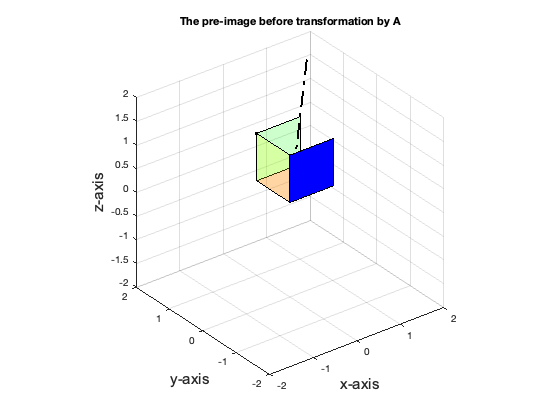
\includegraphics [width=5in]{Problem5_transformation_01.png}
	
	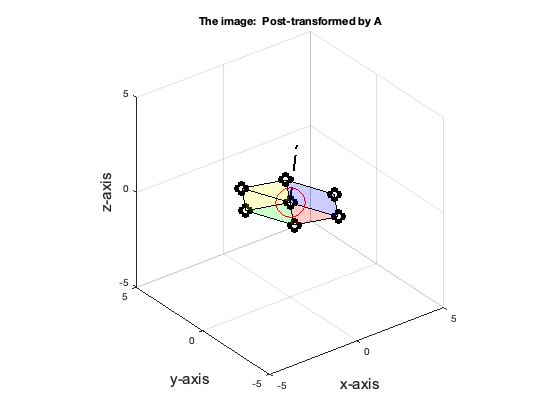
\includegraphics [width=5in]{Problem5_transformation_02.png}
	
\end{center}
\subsection*{C}

If you take the cross product of any two columns of the transformation matrix and normalize it (make it unit length), the output vectors (\(\vec{n_n}\)) will be identical (or in opposite direction \(-\vec{n_n}\)). This demonstrates that they are all in the same plane. Since the matrix we are transforming is a unit cube (or identity matrix \(I\)) then the output of the multiplication is guaranteed to have entries which are all in the plane whose normal is \(\vec{n_n}\), and is proven by the known identity \(A \times I=A\). Calculations below

\begin{verbatim}
	A_1=[2;-1;-1];
	A_2=[-1;2;-1];
	A_3=[-1;-1;2];
	
	C_12 = cross(A_1,A_2);
	C_31 = cross(A_3,A_1);
	C_23 = cross(A_2, A_3);
	
	C_12 = C_12/norm(C_12)
	C_31 = C_31/norm(C_31)
	C_23 = C_23/norm(C_23)
	
	figure;
	hold on;
	grid on;
	
	quiver3(0, 0, 0, A_1(1), A_1(2), A_1(3), 'r', 'LineWidth', 2, 'MaxHeadSize', 0.5);
	quiver3(0, 0, 0, A_2(1), A_2(2), A_2(3), 'g', 'LineWidth', 2, 'MaxHeadSize', 0.5);
	quiver3(0, 0, 0, A_3(1), A_3(2), A_3(3), 'b', 'LineWidth', 2, 'MaxHeadSize', 0.5);
	
	quiver3(0, 0, 0, C_12(1), C_12(2), C_12(3), 'k', 'LineWidth', 2, 'MaxHeadSize', 0.5);
	
	[X, Y] = meshgrid(-2:0.5:2, -2:0.5:2);
	Z = (-C_12(1)*X - C_12(2)*Y) / C_12(3);
	
	surf(X, Y, Z, 'FaceAlpha', 0.3, 'EdgeColor', 'none', 'FaceColor', 'cyan');
	
	xlabel('X'); ylabel('Y'); zlabel('Z');
	title('Vectors A1, A2, A3 and their Normal Vector');
	legend('A1', 'A2', 'A3', 'Normal (C_{12})', 'Plane');
	
	hold off;
	axis equal;
	view(3);
	\end{verbatim}
	
		 \begin{verbatim}
	C_12 =
	
		0.5774
		0.5774
		0.5774
	
	
	C_31 =
	
		0.5774
		0.5774
		0.5774
	
	
	C_23 =
	
		0.5774
		0.5774
		0.5774
	
	\end{verbatim} 
		\centering
	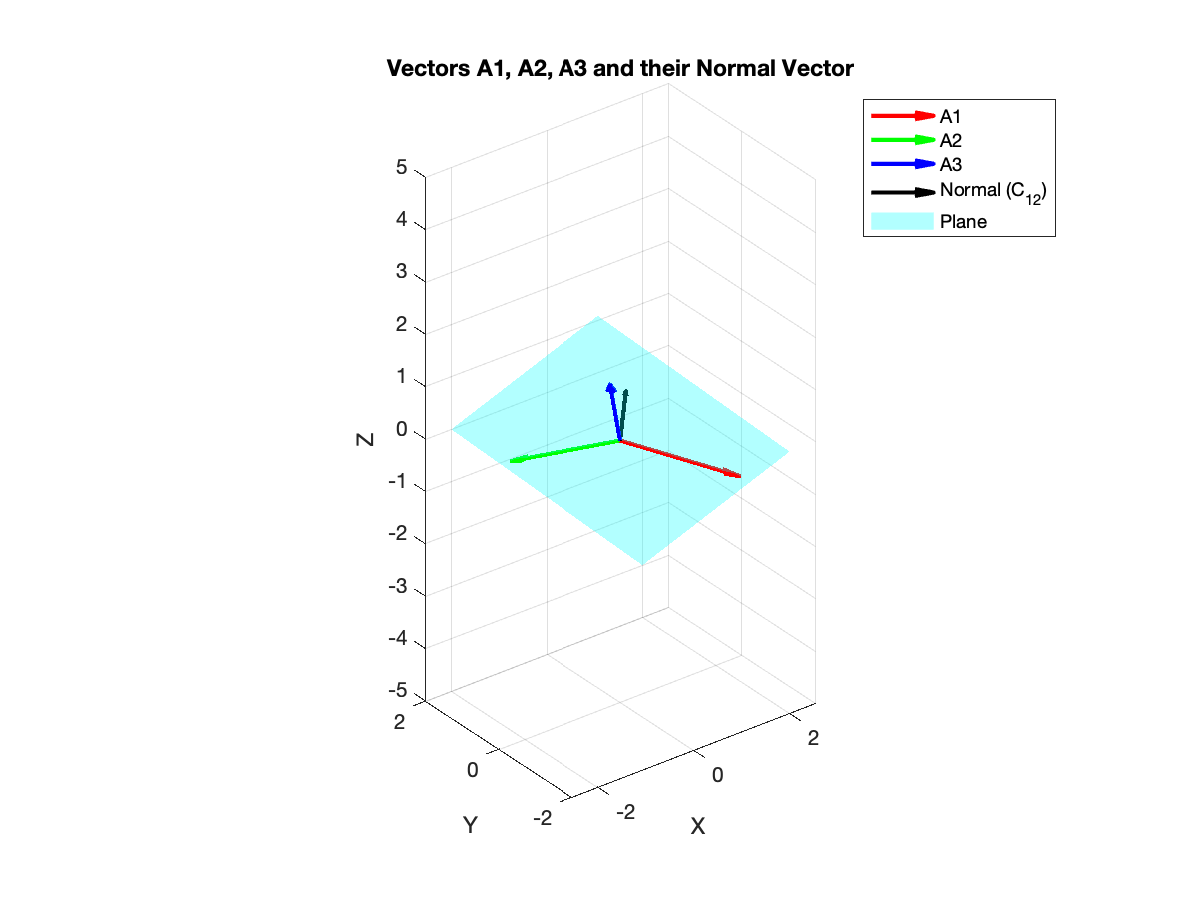
\includegraphics [width=4in]{untitled2_01.eps}
	
	
		
\end{document}